Most of the braille display products available in the market right now, such as those from HumanWare and RNIB, are based on piezoelectric bimorph benders or relay-lever mechanisms.  

The biomorph benders mechanism produces vibrations that move the pin up and down when placed in an electric field. (figure \ref{fig:piezo-bender}, left) In relay-lever mechanisms, when voltage is supplied, the relay pushes the pin up; when the power is off, the self-weight of the lever mechanism lets the pin downward to its original position. (figure \ref{fig:piezo-bender}, right)

\begin{figure} \centering
    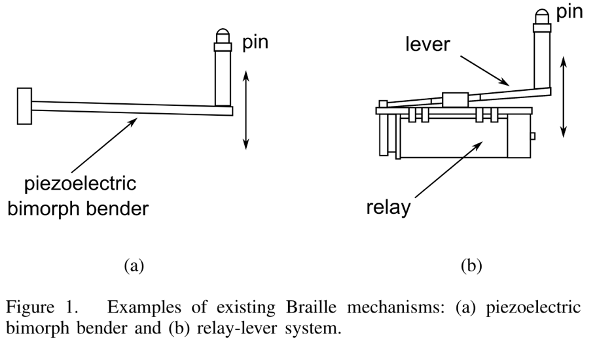
\includegraphics[width=0.6\textwidth]{figures/piezo-bender.png}
\caption{}
\label{fig:piezo-bender}
\end{figure}

The main drawback of these two popular mechanisms is that the functional modules are burdensome and must be placed directly under pins. Therefore, it is hard to make portable devices with these mechanisms and the expensive cost of producing one line of cells also limits the number of lines available. 

Another mechanism that has just been developed recently is piezoelectric ultrasonic motor.
The ultrasonic linear motor consists of a shaft, a mobile element or slider, and a piezoelectric ceramic disk as shown in figure \ref{fig:piezo-miniature}.
The key advantage of this design is the ultra-light weight of this miniature motor.
However, to make a practical tactile display the group developing this proposed a multiplayer solution (figure \ref{fig:piezo-full-design}), which again requires different lines of cells to be far apart. This does not comply with our goal of making a dense tactile display.

\begin{figure} \centering
    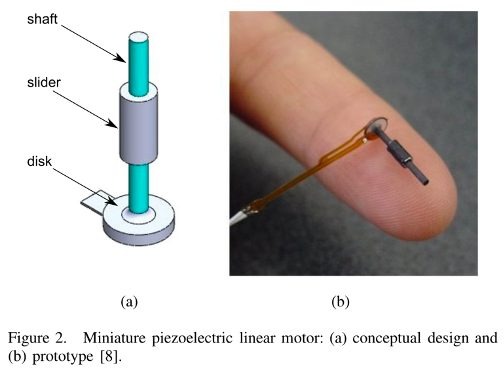
\includegraphics[width=0.6\textwidth]{figures/piezo-miniature.png}
\caption{}
\label{fig:piezo-miniature}
\end{figure}

\begin{figure}\centering
    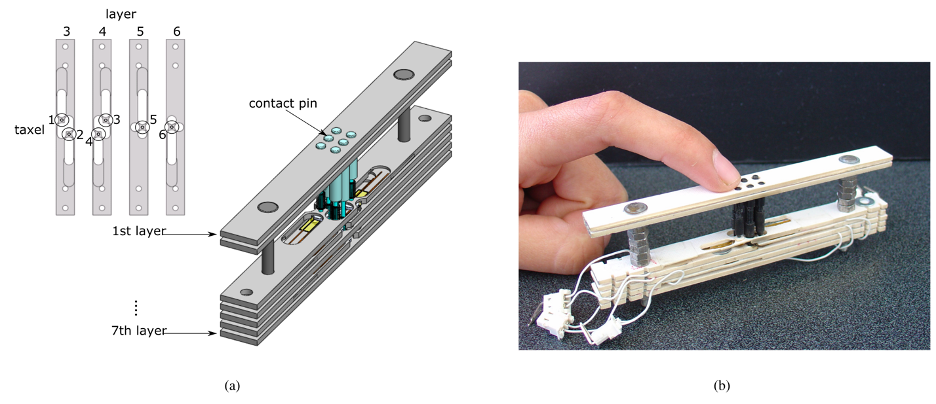
\includegraphics[width=0.6\textwidth]{figures/piezo-full-design.png}
\caption{}
\label{fig:piezo-full-design}
\end{figure}